\chapter{Local memory e sincronizzazione}\label{chap:opencl_lmem}

In questo capitolo si introduce la local memory di OpenCL e i meccanismi di sincronizzazione necessari per usarla correttamente. I concetti vengono presentati in modo progressivo attraverso quattro versioni del kernel \emph{vecsmooth}: scalare, vettoriale, con local memory e vettoriale con local memory.

% =====================================================
\section{Il problema: smoothing di un vettore}\label{sec:opencl_lmem_problema}
% =====================================================

Il problema consiste nel calcolare, per ogni elemento di un vettore di interi, la media tra l'elemento stesso e i suoi vicini immediati:
\[
\texttt{out}[i] = \frac{\texttt{in}[i-1] + \texttt{in}[i] + \texttt{in}[i+1]}{3}
\]
con casi limite agli estremi: il primo elemento usa solo \texttt{in}[0] e \texttt{in}[1], l'ultimo usa \texttt{in}[nels-2] e \texttt{in}[nels-1].

% =====================================================
\section{Versione scalare}\label{sec:opencl_lmem_smooth_base}
% =====================================================

La versione base assegna un work-item per elemento. Usa un accumulatore \texttt{acc} e un divisore \texttt{div} aggiornati solo se l'elemento adiacente esiste, tramite due \texttt{if} indipendenti.

\begin{code}[caption={Kernel smooth scalare}, label={code:smooth_k}]
kernel void smooth_k(global int * restrict out,
                     global const int * restrict in, int nels)
{
    int i = get_global_id(0);
    if (i >= nels) return;

    int acc = in[i];
    int div = 1;

    if (i > 0) {
        acc += in[i-1];
        ++div;
    }
    if (i < nels - 1) {
        acc += in[i+1];
        ++div;
    }

    out[i] = acc/div;
}
\end{code}

Lato host la funzione \texttt{smooth()} calcola la GWS come multiplo della LWS tramite \texttt{round\_mul\_up}:

\begin{code}[caption={Funzione host per il lancio del kernel smooth}, label={code:smooth_host_base}]
cl_event smooth(cl_command_queue que, cl_kernel smooth_k,
    cl_mem out, cl_mem in, cl_int nels,
    size_t lws_cli, cl_event init_evt)
{
    const size_t lws[1] = { lws_cli };
    const size_t gws[1] = { round_mul_up(nels, lws[0]) };

    cl_uint arg_index = 0;
    clSetKernelArg(smooth_k, arg_index++, sizeof(cl_mem), &out);
    clSetKernelArg(smooth_k, arg_index++, sizeof(cl_mem), &in);
    clSetKernelArg(smooth_k, arg_index++, sizeof(nels),   &nels);

    cl_event smooth_evt;
    clEnqueueNDRangeKernel(que, smooth_k, 1, NULL, gws, lws,
                           1, &init_evt, &smooth_evt);
    return smooth_evt;
}
\end{code}

I due \texttt{if} indipendenti per i bordi non sono una scelta arbitraria: la sezione seguente ne spiega il costo rispetto a un \texttt{if}/\texttt{else}.

La versione scalare rilegge gli stessi dati più volte: l'elemento \texttt{in[i]} viene letto dal work-item $i$, ma anche dai work-item $i-1$ e $i+1$ come vicino. Le versioni successive riducono questa ridondanza.

% =====================================================
\section{Costo dei branch: \texttt{if} indipendenti vs \texttt{if}/\texttt{else}}\label{sec:opencl_lmem_branch}
% =====================================================

L'hardware GPU gestisce la divergenza di flusso tramite \emph{predication}: quando i work-item di uno stesso warp seguono percorsi diversi, il hardware esegue tutti i percorsi mascherando selettivamente i work-item che non devono contribuire al risultato.

\noindent
Il costo dipende dalla struttura del condizionale:

\begin{description}
    \item[Due \texttt{if} indipendenti] Ogni condizionale viene valutato separatamente. I work-item che non soddisfano la condizione eseguono comunque le istruzioni del blocco, ma il risultato viene scartato. I due condizionali non si influenzano a vicenda: si paga solo il costo del blocco più costoso tra i due \texttt{if}.

    \item[\texttt{if}/\texttt{else}] Tutti i work-item del wavefront eseguono \emph{entrambi} i rami: prima il blocco \texttt{if} (con i work-item del ramo \texttt{else} mascherati), poi il blocco \texttt{else} (con quelli del ramo \texttt{if} mascherati). Il costo totale è la somma dei due rami.
\end{description}

Ne consegue che due \texttt{if} indipendenti che coprono casi distinti sono preferibili a un \texttt{if}/\texttt{else}: nella forma con \texttt{else} si paga sempre il costo di entrambi i rami.

% =====================================================
\section{Versione vettoriale}\label{sec:opencl_lmem_smooth_v4}
% =====================================================

Nella versione vettoriale ogni work-item opera su una quartina \texttt{int4}. Gli elementi interni della quartina ricevono i loro vicini direttamente dagli altri componenti tramite swizzling, evitando letture ridondanti. Solo gli elementi agli estremi della quartina (\texttt{.x} e \texttt{.w}) devono leggere un elemento dalla quartina adiacente in global memory. Quella lettura usa l'aritmetica dei puntatori per accedere al singolo \texttt{int} senza caricare l'intera quartina.

\begin{code}[caption={Kernel smooth vettoriale con \texttt{int4}}, label={code:smooth_v4_k}]
kernel void smooth_v4_k(global int4 * restrict out,
                        global const int4 * restrict in, int nquarts)
{
    int i = get_global_id(0);
    if (i >= nquarts) return;

    const int4 val = in[i]; /* .x .y .z .w */
    /* vicini interni ottenuti per swizzling */
    int4 acc = val + (int4)(0, val.xyz) + (int4)(val.yzw, 0);
    int4 div = (int4)(2, 3, 3, 2);

    if (i > 0) {
        /* ultimo elemento della quartina precedente */
        acc.x += *((global const int *)(in + i) - 1);
        div.x += 1;
    }
    if (i < nquarts - 1) {
        /* primo elemento della quartina successiva */
        acc.w += *((global const int *)(in + i + 1));
        div.w += 1;
    }

    out[i] = (int4)acc/div;
}
\end{code}

Lato host le differenze rispetto alla versione scalare sono: il numero di quartine \texttt{nels/4} viene passato al kernel al posto di \texttt{nels} (con il vincolo che \texttt{nels} sia multiplo di 4), e il calcolo della banda passante tiene conto che ogni work-item legge 4 elementi propri più 2 di confine e ne scrive 4:

\begin{code}[caption={Differenze host per la versione vettoriale}, label={code:smooth_host_v4}]
/* nels deve essere multiplo di 4 */
cl_event smooth_evt = smooth(que, smooth_k, d_out, d_in,
                              nels/4, lws, init_evt);

/* lettura: 4 propri + 2 di confine; scrittura: 4 */
printf("smooth: %.4gGB/s\n",
       (1 + 6.0/4) * memsize / (double)smooth_ns);
\end{code}

Questa versione accede comunque alla global memory per ogni elemento di confine. La sezione seguente introduce la local memory, che permette di condividere dati tra work-item dello stesso work-group senza tornare alla global memory.

% =====================================================
\section{La local memory}\label{sec:opencl_lmem_concetto}
% =====================================================

La local memory (chiamata \emph{shared memory} in CUDA) è una memoria on-chip allocata per ogni work-group al momento del lancio del kernel. A differenza della global memory, che persiste per l'intera durata del programma, la local memory è temporanea: viene allocata quando il work-group inizia l'esecuzione e viene liberata quando termina.

\noindent
Le proprietà principali sono:
\begin{itemize}
    \item È visibile solo ai work-item dello stesso work-group; work-group diversi hanno aree di local memory distinte e non possono comunicare tra loro tramite essa.
    \item Ha latenza molto inferiore alla global memory, poiché si trova fisicamente sulla stessa compute unit che esegue il work-group.
    \item La sua dimensione è limitata e influenza quanti work-group possono essere attivi contemporaneamente sulla stessa compute unit.
\end{itemize}

L'utilità principale è che i work-item dello stesso work-group girano sulla stessa compute unit: possono quindi condividere dati tramite la local memory senza passare dalla global memory, che ha latenza elevata.

Nel codice device si dichiara con la keyword \texttt{\_\_local} (o \texttt{local}):

\begin{code}[caption={Dichiarazione di un parametro in local memory}, label={code:lmem_decl}]
kernel void esempio_k(local int * restrict cache)
{
    /* cache: local memory, condivisa tra tutti i WI del work-group */
}
\end{code}

% =====================================================
\section{Indici locali: \texttt{get\_local\_id()} e \texttt{get\_local\_size()}}\label{sec:opencl_lmem_ids}
% =====================================================

Oltre all'indice globale, ogni work-item ha un indice \emph{locale} che lo identifica all'interno del proprio work-group:

\begin{description}
    \item[\texttt{get\_global\_id(0)}] Indice del work-item nella griglia globale, da \texttt{0} a \texttt{GWS\,-\,1}.
    \item[\texttt{get\_local\_id(0)}] Indice del work-item all'interno del suo work-group, da \texttt{0} a \texttt{LWS\,-\,1}.
    \item[\texttt{get\_local\_size(0)}] Dimensione del work-group (= LWS).
\end{description}

\paragraph{Esempio.} Con GWS\,$=8$ e LWS\,$=4$ si hanno due work-group:
\begin{itemize}
    \item WG\,0: \texttt{gi} $= 0,1,2,3$ \quad \texttt{li} $= 0,1,2,3$
    \item WG\,1: \texttt{gi} $= 4,5,6,7$ \quad \texttt{li} $= 0,1,2,3$
\end{itemize}

L'indice locale è fondamentale per posizionare i dati nella cache condivisa: il work-item con \texttt{li}$= k$ scrive il proprio valore in \texttt{cache[k+1]} e può leggere quello del vicino in \texttt{cache[k]} e \texttt{cache[k+2]} (con l'offset di 1 della cache lws$+$2 descritta nella sezione seguente).

% =====================================================
\section{Trade-off nella dimensione della cache}\label{sec:opencl_lmem_tradeoff}
% =====================================================

Per il kernel smooth, ogni work-item ha bisogno del proprio elemento e dei due elementi adiacenti. Esistono due scelte per la dimensione della cache:

\begin{description}
    \item[Cache di lws$+$2 elementi] Si riserva uno slot prima del primo elemento e uno dopo l'ultimo del work-group. Il vantaggio è che il kernel legge sempre dalla cache con un accesso uniforme; lo svantaggio è un'inizializzazione più complessa, in cui il primo e l'ultimo work-item devono caricare elementi aggiuntivi dalla global memory.

    \item[Cache di lws elementi] Ogni work-item scrive solo il proprio dato. L'inizializzazione è semplice, ma i work-item ai bordi del work-group devono ancora accedere alla global memory per il vicino esterno.
\end{description}

Nelle implementazioni che seguono si adotta la prima alternativa (lws$+$2): il kernel legge sempre dalla cache, rendendo il comportamento uniforme per tutti i work-item.

% =====================================================
\section{Race condition in local memory}\label{sec:opencl_lmem_race}
% =====================================================

I work-item dello stesso work-group sono garantiti in esecuzione contemporanea sulla stessa compute unit, ma non necessariamente sulla stessa istruzione nello stesso ciclo di clock. L'hardware li raggruppa in wavefront di dimensione fissa — tipicamente 32 o 64 work-item — e work-item appartenenti a wavefront diversi possono trovarsi in punti diversi del programma.

Se un work-group ha LWS $>$ warp\_size, esso è composto da più wavefront. In questo caso è possibile una \emph{race condition}: un work-item di un wavefront potrebbe leggere dalla local memory un valore che un work-item di un altro wavefront non ha ancora scritto.

\paragraph{Esempio.} Con LWS\,$=64$ e warp\_size\,$=32$, un work-group è composto da 2 wavefront. Il wavefront~0 (work-item 0--31) potrebbe avanzare all'istruzione di lettura dalla cache prima che il wavefront~1 (work-item 32--63) abbia completato le scritture. Il valore letto sarebbe indeterminato.

La soluzione è inserire una barriera di sincronizzazione tra la fase di scrittura e quella di lettura della cache.

% =====================================================
\section{Barriere}\label{sec:opencl_lmem_barrier}
% =====================================================

\begin{code}[caption={Barriera di sincronizzazione sulla local memory}, label={code:barrier}]
barrier(CLK_LOCAL_MEM_FENCE);
\end{code}

La semantica è la seguente: tutte le scritture in local memory effettuate \emph{prima} della barriera da qualsiasi work-item del work-group sono garantite visibili a \emph{tutti} i work-item dello stesso work-group \emph{dopo} la barriera. Nessun work-item può superare la barriera finché tutti gli altri non la raggiungono.

La barriera ha due vincoli importanti:

\begin{enumerate}
    \item \textbf{Solo intra-work-group.} Non esiste una barriera a livello di griglia: work-group diversi non possono sincronizzarsi tra loro e non è garantito che siano nemmeno in esecuzione contemporaneamente.

    \item \textbf{Tutti i work-item devono raggiungerla.} Se alcuni work-item escono dal kernel prima della barriera (ad esempio con un \texttt{return} anticipato), gli altri rimarranno in attesa indefinita. Il pattern corretto è spostare il controllo \texttt{if (gi >= nels) return;} \emph{dopo} la barriera.
\end{enumerate}

% =====================================================
\section{Allocazione di local memory dall'host}\label{sec:opencl_lmem_alloc}
% =====================================================

La local memory non viene allocata nel codice device: è l'host a specificarne la dimensione tramite \texttt{clSetKernelArg}, passando \texttt{NULL} come valore:

\begin{code}[caption={Allocazione di local memory dall'host}, label={code:lmem_host_alloc}]
err = clSetKernelArg(smooth_k, arg_index,
                     (lws_cli + 2) * sizeof(cl_int), NULL);
\end{code}

Il \texttt{NULL} indica al runtime di allocare il numero di byte specificato come local memory per ciascun work-group, senza inizializzarli. La dimensione della cache influenza l'occupazione della compute unit: più grande è la cache, minore è il numero di work-group che possono essere attivi contemporaneamente sulla stessa CU, riducendo il margine per nascondere la latenza delle letture dalla global memory.

% =====================================================
\section{Versione con local memory}\label{sec:opencl_lmem_smooth_lmem}
% =====================================================

In questa versione ogni work-item carica il proprio elemento in una cache condivisa di \texttt{lws+2} elementi. Il primo work-item del work-group carica anche il predecessore del work-group, l'ultimo carica anche il successore. Una barriera garantisce che la cache sia completamente inizializzata prima che qualsiasi work-item la legga.

Il \texttt{return} anticipato per gli indici fuori range viene spostato \emph{dopo} la barriera, in modo che tutti i work-item del work-group la raggiungano.

\begin{code}[caption={Kernel smooth con local memory}, label={code:smooth_lmem_k}]
kernel void smooth_lmem_k(global int * restrict out,
                          global const int * restrict in,
                          int nels,
                          local int * restrict cache)
{
    const int lws = get_local_size(0);
    int gi = get_global_id(0);
    int li = get_local_id(0);

    int val, acc;
    int div = 1;

    if (gi < nels) {
        int val = in[gi];
        cache[li + 1] = val; /* elemento centrale */

        /* il primo WI del WG carica il predecessore del WG */
        if (li == 0 && gi != 0)
            cache[0] = in[gi - 1];
        /* l'ultimo WI del WG carica il successore del WG */
        if (li == lws - 1 && gi < nels - 1)
            cache[li + 2] = in[gi + 1];

        acc = val;
    }

    barrier(CLK_LOCAL_MEM_FENCE); /* tutte le scritture in cache completate */

    if (gi >= nels) return; /* return DOPO la barriera */

    if (gi > 0) {
        acc += cache[li];     /* predecessore dalla cache */
        ++div;
    }
    if (gi < nels - 1) {
        acc += cache[li + 2]; /* successore dalla cache */
        ++div;
    }

    out[gi] = acc/div;
}
\end{code}

Lato host l'unica differenza rispetto alla versione scalare è l'argomento della cache, allocato con \texttt{NULL}:

\begin{code}[caption={Allocazione della cache lato host (versione lmem)}, label={code:smooth_host_lmem}]
clSetKernelArg(smooth_k, arg_index++,
               (lws_cli + 2) * sizeof(cl_int), NULL);
\end{code}

% =====================================================
\section{Versione vettoriale con local memory}\label{sec:opencl_lmem_smooth_v4lmem}
% =====================================================

L'ultima versione combina vettorizzazione e local memory. Poiché ogni work-item opera su una quartina, gli unici elementi che possono essere utili ai work-item vicini sono il primo (\texttt{.x}) e l'ultimo (\texttt{.w}) componente di ciascuna quartina.
Considerando che non vi è alcun elemento che possa fungere sia da precedente che da successivo, si usano due cache separate di \texttt{lws} elementi ciascuna:

\begin{itemize}
    \item \texttt{cache\_prec[li]}: contiene l'ultimo elemento (\texttt{.w}) della quartina del work-item \texttt{li-1}, ovvero il predecessore della quartina del work-item \texttt{li}.
    \item \texttt{cache\_succ[li]}: contiene il primo elemento (\texttt{.x}) della quartina del work-item \texttt{li+1}, ovvero il successore della quartina del work-item \texttt{li}.
\end{itemize}

Il primo work-item del work-group non ha un predecessore in \texttt{cache\_prec} e lo carica dalla global memory; l'ultimo non ha un successore in \texttt{cache\_succ} e lo carica anch'esso dalla global memory.

\begin{code}[caption={Kernel smooth vettoriale con local memory}, label={code:smooth_v4_lmem_k}]
kernel void smooth_v4_lmem_k(global int4 * restrict out,
                              global const int4 * restrict in,
                              int nquarts,
                              local int * restrict cache_prec,
                              local int * restrict cache_succ)
{
    int gi = get_global_id(0);
    int li = get_local_id(0);
    const int lws = get_local_size(0);

    const int4 val = gi < nquarts ? in[gi] : (int4)(0);

    /* ogni WI fornisce il suo .w al successivo (cache_prec)
       e il suo .x al precedente (cache_succ) */
    if (li + 1 < lws) cache_prec[li + 1] = val.w;
    if (li > 0)       cache_succ[li - 1] = val.x;

    /* il primo WI del WG legge il predecessore dalla global memory */
    if (gi > 0 && li == 0)
        cache_prec[0] = *((global const int *)(in + gi) - 1);
    /* l'ultimo WI del WG legge il successore dalla global memory */
    if (gi < nquarts - 1 && li == lws - 1)
        cache_succ[li] = *((global const int *)(in + gi + 1));

    barrier(CLK_LOCAL_MEM_FENCE);

    int4 acc = val + (int4)(0, val.xyz) + (int4)(val.yzw, 0);
    int4 div = (int4)(2, 3, 3, 2);

    if (gi > 0) {
        acc.x += cache_prec[li];
        div.x += 1;
    }
    if (gi < nquarts - 1) {
        acc.w += cache_succ[li];
        div.w += 1;
    }

    if (gi < nquarts) out[gi] = acc/div;
}
\end{code}

Lato host si allocano due cache di \texttt{lws\_cli} elementi ciascuna — senza il \texttt{+2} della versione scalare — poiché le cache contengono esattamente un elemento per work-item. Come nella versione vettoriale base, si passa \texttt{nels/4} al kernel:

\begin{code}[caption={Allocazione delle due cache lato host (versione v4+lmem)}, label={code:smooth_host_v4lmem}]
clSetKernelArg(smooth_k, arg_index++, lws_cli * sizeof(cl_int), NULL);
clSetKernelArg(smooth_k, arg_index++, lws_cli * sizeof(cl_int), NULL);

/* nels deve essere multiplo di 4 */
cl_event smooth_evt = smooth(que, smooth_k, d_out, d_in,
                              nels/4, lws, init_evt);
\end{code}

% =====================================================
\section{Trasposizione di una matrice}\label{sec:opencl_lmem_transpose}
% =====================================================

La trasposizione di una matrice $R \times C$ produce una matrice $C \times R$ in cui l'elemento in posizione $(r,\,c)$ nella matrice originale compare in posizione $(c,\,r)$ nella trasposta. L'implementazione più naturale (imbarazzantemente parallela) assegna un work-item per elemento della trasposta, usando \texttt{get\_global\_id(0)} per la colonna (asse rapido) e \texttt{get\_global\_id(1)} per la riga.

\begin{code}[caption={Kernel naive di trasposizione}, label={code:transpose_naive}]
/* t_rows, t_cols: righe e colonne della trasposta */
kernel void transpose_k(global int * restrict trasposta,
                        global const int * restrict originale,
                        int t_rows, int t_cols)
{
    int t_c = get_global_id(0); /* colonna della trasposta */
    int t_r = get_global_id(1); /* riga della trasposta */

    if (t_r < t_rows && t_c < t_cols)
        trasposta[t_r * t_cols + t_c] = originale[t_c * t_rows + t_r];
}
\end{code}

La coalescenza degli accessi è asimmetrica:

\begin{description}
    \item[Scritture] L'indice lineare \texttt{t\_r\,*\,t\_cols\,+\,t\_c} varia di~1 al variare di \texttt{t\_c} (asse~0, il più rapido): le scritture su \texttt{trasposta} sono coalescenti.

    \item[Letture] L'indice lineare \texttt{t\_c\,*\,t\_rows\,+\,t\_r} varia di \texttt{t\_rows} al variare di \texttt{t\_c}: le letture da \texttt{originale} hanno stride pari al numero di righe dell'originale e non sono coalescenti.
\end{description}

Invertendo gli assi --- \texttt{get\_global\_id(0)} per la riga, \texttt{get\_global\_id(1)} per la colonna --- si ottiene la situazione opposta: letture coalescenti ma scritture non coalescenti. In entrambe le varianti uno dei due accessi ha stride.

\begin{figure}[htbp]
\centering
\resizebox{0.82\textwidth}{!}{%
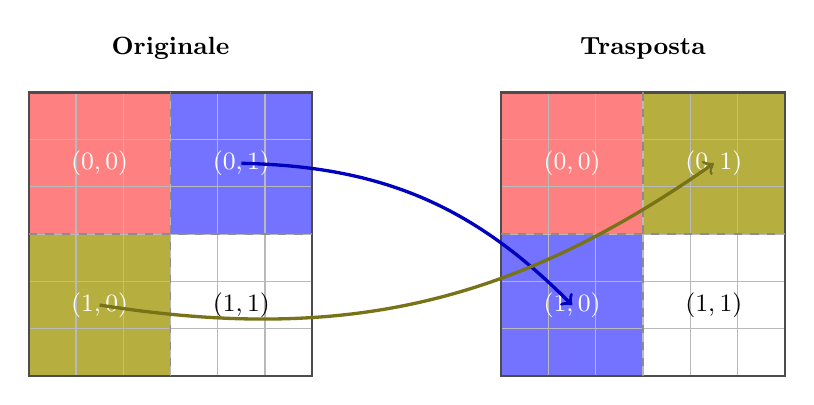
\begin{tikzpicture}[x=0.6cm, y=0.6cm]

%% ---- Matrice originale (x=[0,6], y=[0,-6]) ----
\fill[red!50]   (0, 0) rectangle (3,-3);
\fill[blue!55]  (3, 0) rectangle (6,-3);
\fill[olive!65] (0,-3) rectangle (3,-6);
\foreach \c in {0,...,6} \draw[gray!55, thin] (\c,0)--(\c,-6);
\foreach \r in {0,...,6} \draw[gray!55, thin] (0,-\r)--(6,-\r);
\draw[black!70, thick] (0,0) rectangle (6,-6);
\draw[black!45, semithick, dashed] (3,0)--(3,-6);
\draw[black!45, semithick, dashed] (0,-3)--(6,-3);
\node[above, font=\small\bfseries] at (3,0.5) {Originale};
\node[font=\small\bfseries, text=white]  at (1.5,-1.5) {$(0,0)$};
\node[font=\small\bfseries, text=white]  at (4.5,-1.5) {$(0,1)$};
\node[font=\small\bfseries, text=white]  at (1.5,-4.5) {$(1,0)$};
\node[font=\small\bfseries]              at (4.5,-4.5) {$(1,1)$};

%% ---- Matrice trasposta (x=[10,16], y=[0,-6]) ----
\fill[red!50]   (10, 0) rectangle (13,-3);
\fill[olive!65] (13, 0) rectangle (16,-3);
\fill[blue!55]  (10,-3) rectangle (13,-6);
\foreach \c in {0,...,6} \draw[gray!55, thin] ({10+\c},0)--({10+\c},-6);
\foreach \r in {0,...,6} \draw[gray!55, thin] (10,-\r)--(16,-\r);
\draw[black!70, thick] (10,0) rectangle (16,-6);
\draw[black!45, semithick, dashed] (13,0)--(13,-6);
\draw[black!45, semithick, dashed] (10,-3)--(16,-3);
\node[above, font=\small\bfseries] at (13,0.5) {Trasposta};
\node[font=\small\bfseries, text=white]  at (11.5,-1.5) {$(0,0)$};
\node[font=\small\bfseries, text=white]  at (14.5,-1.5) {$(0,1)$};
\node[font=\small\bfseries, text=white]  at (11.5,-4.5) {$(1,0)$};
\node[font=\small\bfseries]              at (14.5,-4.5) {$(1,1)$};

%% ---- Frecce tra blocchi fuori diagonale ----
\draw[->, blue!75!black, very thick, bend left=22]
    (4.5,-1.5) to (11.5,-4.5);
\draw[->, olive!80!black, very thick, bend right=22]
    (1.5,-4.5) to (14.5,-1.5);

\end{tikzpicture}
}
\caption{Trasposizione di una matrice $6\times6$ con blocchi $3\times3$ (\texttt{lws}$=3$, quattro work-group). Le coordinate $(g_r,\,g_c)$ identificano il blocco nella griglia di work-group. I blocchi diagonali rimangono in posizione; i blocchi fuori diagonale si scambiano. Ciascun blocco corrisponde al tile elaborato da un work-group.}
\label{fig:trasposizione_blocchi}
\end{figure}

Il benchmark misura la banda passante come $2 \times \texttt{memsize}$: si legge l'intera matrice originale e si scrive l'intera trasposta.

% =====================================================
\section{Letture coalescenti vs scritture coalescenti}\label{sec:opencl_lmem_coal_rw}
% =====================================================

Quando non è possibile avere entrambi gli accessi coalescenti, conviene privilegiare le \emph{letture}. Le scritture in memoria non possono iniziare finché le letture necessarie non sono terminate: il tempo di lettura è sul percorso critico, quello di scrittura no. Ottimizzare le letture riduce quindi direttamente la latenza complessiva del kernel.

Tuttavia, anche nel caso ottimale con letture coalescenti, il kernel naive lascia le scritture con stride. La local memory consente di eliminare lo stride su \emph{entrambi} gli accessi.

% =====================================================
\section{Trasposizione con tile in local memory}\label{sec:opencl_lmem_transpose_tile}
% =====================================================

L'idea è dividere la matrice in \emph{tile} quadrati di \texttt{lws}$\times$\texttt{lws} elementi, uno per work-group. Ogni work-group esegue tre fasi:

\begin{enumerate}
    \item Carica il proprio tile dall'originale nella local memory con \emph{letture coalescenti}.
    \item Sincronizza con una barriera.
    \item Scrive il tile nella posizione trasposta della matrice risultato con \emph{scritture coalescenti}, leggendo dalla local memory con gli indici locali scambiati.
\end{enumerate}

\paragraph{Fase~1 (caricamento).} Il work-item con indici locali $(l_c,\,l_r)$ nel work-group $(g_c,\,g_r)$ legge dall'originale la posizione globale $(\text{orig\_r}, \text{orig\_c}) = (g_r \cdot \texttt{lws} + l_r,\; g_c \cdot \texttt{lws} + l_c)$. Al variare di $l_c$ (asse~0), l'indice lineare $\text{orig\_r} \cdot C + \text{orig\_c}$ varia di~1: le letture sono coalescenti. Il valore viene scritto in \texttt{tile[$l_r \cdot \texttt{lws} + l_c$]}.

\paragraph{Fase~2 (scrittura).} Il work-group che ha letto il blocco $(g_r, g_c)$ dell'originale scrive nel blocco $(g_c, g_r)$ della trasposta (coordinate di work-group scambiate). Ogni work-item $(l_c,\,l_r)$ legge \texttt{tile[$l_c \cdot \texttt{lws} + l_r$]} (indici locali scambiati rispetto alla fase~1) e scrive in posizione $(\text{trans\_r}, \text{trans\_c}) = (g_c \cdot \texttt{lws} + l_r,\; g_r \cdot \texttt{lws} + l_c)$. Al variare di $l_c$ (asse~0), l'indice lineare $\text{trans\_r} \cdot R + \text{trans\_c}$ varia di~1: le scritture sono coalescenti.

\begin{figure}[htbp]
\centering
% Ridotto a 0.85 per renderlo più piccolo e gestibile
\resizebox{0.85\textwidth}{!}{%
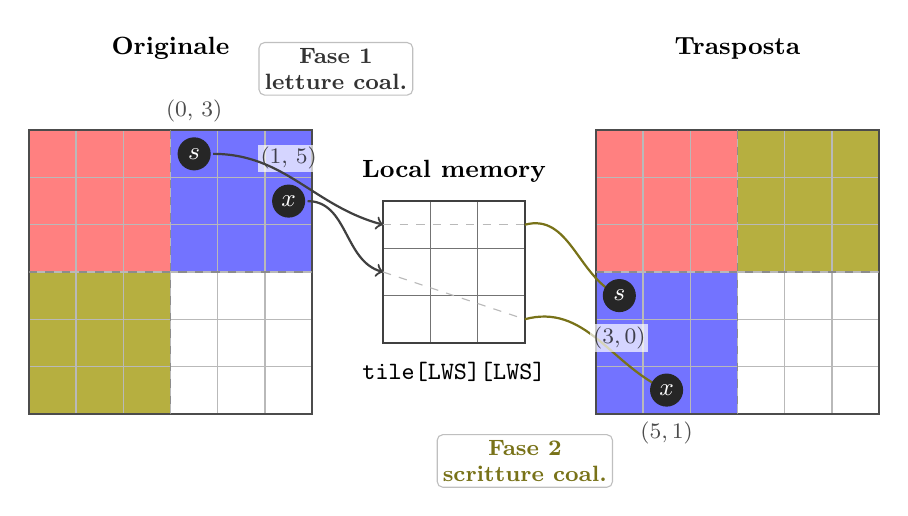
\begin{tikzpicture}[x=0.6cm, y=0.6cm]

%% ---- Matrice originale (x=[0,6]) ----
\fill[red!50]   (0, 0) rectangle (3,-3);
\fill[blue!55]  (3, 0) rectangle (6,-3);
\fill[olive!65] (0,-3) rectangle (3,-6);
\foreach \c in {0,...,6} \draw[gray!55, thin] (\c,0)--(\c,-6);
\foreach \r in {0,...,6} \draw[gray!55, thin] (0,-\r)--(6,-\r);
\draw[black!70, thick] (0,0) rectangle (6,-6);
\draw[black!45, semithick, dashed] (3,0)--(3,-6);
\draw[black!45, semithick, dashed] (0,-3)--(6,-3);
\node[above, font=\small\bfseries] at (3,1.3) {Originale};

%% ---- Etichetta Fase 1 (Spostata più vicina alla matrice originale) ----
\node[font=\footnotesize\bfseries, black!80, align=center,
      draw=gray!50, fill=white, inner sep=2pt, rounded corners=2pt]
    at (6.5, 1.3) {Fase~1\\ letture coal.};

%% ---- Tile (local memory): x=[7.5,10.5], y=[-1.5,-4.5] ----
\fill[white] (7.5,-1.5) rectangle (10.5,-4.5);
\foreach \c in {0,...,3} \draw[black!55, thin] ({7.5+\c},-1.5)--({7.5+\c},-4.5);
\foreach \r in {0,...,3} \draw[black!55, thin] (7.5,{-1.5-\r})--(10.5,{-1.5-\r});
\draw[black!75, thick] (7.5,-1.5) rectangle (10.5,-4.5);
\node[above, font=\small\bfseries] at (9,-1.3) {Local memory};
\node[below, font=\small] at (9,-4.7) {\texttt{tile[LWS][LWS]}};

%% ---- Matrice trasposta (x=[12,18]) ----
\fill[red!50]   (12, 0) rectangle (15,-3);
\fill[olive!65] (15, 0) rectangle (18,-3);
\fill[blue!55]  (12,-3) rectangle (15,-6);
\foreach \c in {0,...,6} \draw[gray!55, thin] ({12+\c},0)--({12+\c},-6);
\foreach \r in {0,...,6} \draw[gray!55, thin] (12,-\r)--(18,-\r);
\draw[black!70, thick] (12,0) rectangle (18,-6);
\draw[black!45, semithick, dashed] (15,0)--(15,-6);
\draw[black!45, semithick, dashed] (12,-3)--(18,-3);
\node[above, font=\small\bfseries] at (15,1.3) {Trasposta};

%% ---- Elemento s: (r=0, c=3) ----
\fill[black!85] (3.5,-0.5) circle (0.35);
\node[font=\small\bfseries, white] at (3.5,-0.5) {$s$};
\node[above, font=\footnotesize, fill=white, fill opacity=0.7, inner sep=1pt] 
    at (3.5, 0.1) {$(0,\,3)$};

%% Elemento x: (r=1, c=5) ----
\fill[black!85] (5.5,-1.5) circle (0.35);
\node[font=\small\bfseries, white] at (5.5,-1.5) {$x$};
\node[above, font=\footnotesize, fill=white, fill opacity=0.7, inner sep=1pt] 
    at (5.5,-0.9) {$(1,\,5)$};

%% ---- Frecce load ----
\draw[->, thick, black!75] (3.9,-0.5) to[out=0, in=165] (7.5,-2);
\draw[->, thick, black!75] (5.9,-1.5) to[out=0, in=165] (7.5,-3);

%% ---- Percorso nella tile ----
\draw[gray!55, thin, dashed] (7.5,-2) -- (10.5,-2);
\draw[gray!55, thin, dashed] (7.5,-3) -- (10.5,-4);

%% ---- Etichetta Fase 2 ----
\node[font=\footnotesize\bfseries, olive!80!black, align=center,
      draw=gray!50, fill=white, inner sep=2pt, rounded corners=2pt]
    at (10.5,-7.0) {Fase~2\\ scritture coal.};

%% ---- Frecce store ----
\draw[->, thick, olive!80!black] (10.5,-2) to[out=15, in=155] (12.5,-3.5);
\draw[->, thick, olive!80!black] (10.5,-4) to[out=15, in=155] (13.5,-5.5);

%% ---- Elementi nella trasposta ----
\fill[black!85] (12.5,-3.5) circle (0.35);
\node[font=\small\bfseries, white] at (12.5,-3.5) {$s$};
\node[below, font=\footnotesize, fill=white, fill opacity=0.7, inner sep=1pt] 
    at (12.5,-4.1) {$(3, 0)$};

\fill[black!85] (13.5,-5.5) circle (0.35);
\node[font=\small\bfseries, white] at (13.5,-5.5) {$x$};
\node[below, font=\footnotesize, fill=white, fill opacity=0.7, inner sep=1pt] 
    at (13.5,-6.1) {$(5, 1)$};

\end{tikzpicture}
}
\caption{Trasposizione con tile in local memory. Si tracciano due elementi del blocco blu: $s\,(0,3)$ (diagonale del tile, $l_c=l_r=0$) e $x\,(1,5)$ (fuori diagonale, $l_r=1,\,l_c=2$). Le frecce scure mostrano la \emph{Fase~1} (letture coalescenti dall'originale al tile); le linee tratteggiate il percorso interno al tile (orizzontale per $s$, diagonale per $x$ — lo scambio $r\!\leftrightarrow\!c$ avviene qui); le frecce dorate la \emph{Fase~2} (scritture coalescenti verso la trasposta). Le coordinate $(r,c)$ si scambiano: $(0,3)\!\to\!(3,0)$ e $(1,5)\!\to\!(5,1)$.}
\label{fig:trasposizione_tile}
\end{figure}

In sintesi, in fase~2 ogni work-item scrive il valore che, in fase~1, è stato letto dal work-item con indici locali scambiati $(l_r, l_c)$. La dimensione del tile è un trade-off: più è grande, più si riduce il numero di blocchi fuori diagonale (quelli con accessi non coalescenti) e più si aumenta la banda passante; ma più è grande, meno work-group possono essere attivi contemporaneamente sulla stessa compute unit, riducendo l'occupazione e la capacità di nascondere la latenza delle letture dalla global memory. Tipicamente si sceglie \texttt{lws} pari alla dimensione del warp/wavefront (32 o 64).

\begin{code}[caption={Kernel di trasposizione con tile in local memory}, label={code:transpose_lmem}]

/* Richiede orig_rows e orig_cols multipli di lws */
kernel void transpose_lmem_k(global int * restrict trasposta,
                              global const int * restrict originale,
                              int orig_rows, int orig_cols,
                              local int * restrict tile)
{
    int li_c = get_local_id(0);
    int li_r = get_local_id(1);
    int lws  = get_local_size(0); /* work-group quadrato */

    int orig_c = get_group_id(0) * lws + li_c;
    int orig_r = get_group_id(1) * lws + li_r;

    /* Fase 1: caricamento con letture coalescenti */
    tile[li_r * lws + li_c] = originale[orig_r * orig_cols + orig_c];

    barrier(CLK_LOCAL_MEM_FENCE);

    /* Fase 2: work-group trasposto, indici locali scambiati */
    int trans_r = get_group_id(0) * lws + li_r;
    int trans_c = get_group_id(1) * lws + li_c;

    trasposta[trans_r * orig_rows + trans_c] = tile[li_c * lws + li_r];
}
\end{code}

Le coordinate del work-group sono scambiate tra le due fasi: \texttt{get\_group\_id(0)} contribuisce all'indice di riga nella fase~2 anziché di colonna come nella fase~1. Gli indici locali $(l_c, l_r)$ mantengono invece la loro direzione rispetto agli assi. Se \texttt{get\_group\_id()} non fosse disponibile, si ricava come \texttt{get\_global\_id(d)\,/\,get\_local\_size(d)}.

Lato host la differenza rispetto agli altri kernel è la griglia bidimensionale e l'allocazione del tile come local memory:

\begin{code}[caption={Lancio del kernel di trasposizione con tile}, label={code:transpose_host}]
const size_t lws[2] = { lws_cli, lws_cli }; /* work-group quadrato */
const size_t gws[2] = { round_mul_up(orig_cols, lws[0]),
                         round_mul_up(orig_rows, lws[1]) };

cl_uint arg = 0;
clSetKernelArg(k, arg++, sizeof(cl_mem), &trasposta);
clSetKernelArg(k, arg++, sizeof(cl_mem), &originale);
clSetKernelArg(k, arg++, sizeof(cl_int), &orig_rows);
clSetKernelArg(k, arg++, sizeof(cl_int), &orig_cols);
clSetKernelArg(k, arg++, lws_cli * lws_cli * sizeof(cl_int), NULL);

clEnqueueNDRangeKernel(que, k, 2, NULL, gws, lws, ...);

/* benchmark: lettura originale + scrittura trasposta = 2 * memsize */
printf("transpose: %.4gGB/s\n", 2.0 * memsize / (double)ns);
\end{code}

% =====================================================
\section{Bank conflict nella local memory}\label{sec:opencl_lmem_bank_conflict}
% =====================================================

La local memory è fisicamente realizzata con \emph{banchi} di memoria su chip: strutture di 32~bit (un intero) indirizzate in modo \emph{trasversale}, ovvero indirizzi consecutivi cadono su banchi consecutivi. In questo schema ogni colonna del tile (con indice fisico~$c$) corrisponde al banco $c \bmod N_b$, dove $N_b$ è il numero di banchi (tipicamente~32).

\begin{description}
    \item[Accessi ottimali] Work-item diversi dello stesso sottogruppo che accedono a \emph{banchi diversi} vengono serviti in un unico ciclo di clock.

    \item[Bank conflict] Se due work-item dello stesso sottogruppo richiedono lo \emph{stesso banco}, gli accessi vengono serializzati: il banco risponde a un work-item alla volta, con un ciclo di clock aggiuntivo per ogni conflitto.

    \item[Broadcast] Eccezione: se tutti i work-item leggono lo stesso identico indirizzo, la local memory invia il dato in broadcast senza alcun conflitto.
\end{description}

Analizziamo il kernel \texttt{transpose\_lmem\_k} con $\texttt{lws} = 32$. Nella \emph{fase~1} l'indice fisico è \texttt{tile[li\_r*lws\,+\,li\_c]}: al variare di \texttt{li\_c} il banco vale $(\texttt{li\_r}\cdot 32 + \texttt{li\_c}) \bmod 32 = \texttt{li\_c}$, quindi ogni work-item accede a un banco diverso (nessun conflitto). Nella \emph{fase~2} l'indice diventa \texttt{tile[li\_c*lws\,+\,li\_r]}: al variare di \texttt{li\_c} il banco vale $(\texttt{li\_c}\cdot 32 + \texttt{li\_r}) \bmod 32 = \texttt{li\_r}$, costante per tutti i work-item. Tutti accedono allo stesso banco~$\texttt{li\_r}$: \textbf{bank conflict}.

\begin{figure}[htbp]
\centering
\resizebox{0.84\textwidth}{!}{%
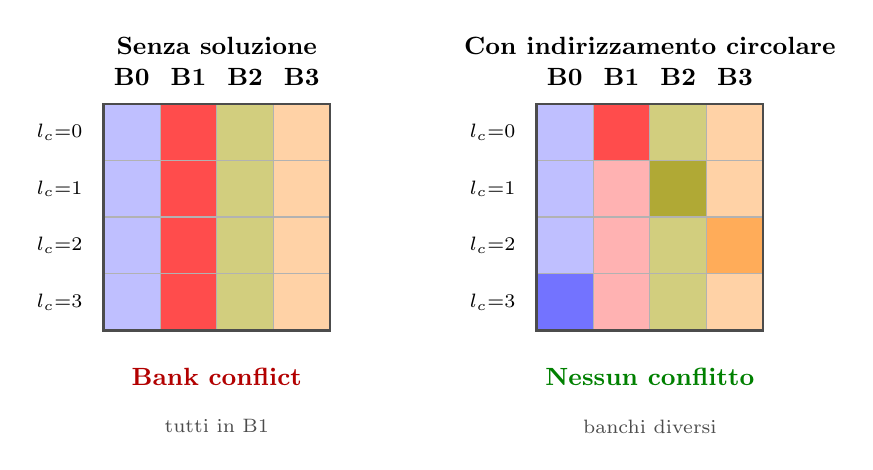
\begin{tikzpicture}[x=0.72cm, y=0.72cm]

%% === PANNELLO SINISTRO: bank conflict ===
\fill[blue!25]   (0, 0) rectangle (1,-4);
\fill[red!30]    (1, 0) rectangle (2,-4);
\fill[olive!40]  (2, 0) rectangle (3,-4);
\fill[orange!35] (3, 0) rectangle (4,-4);

%% Fase 2 con li_r=1: tile[li_c*4+1] → tutte nella colonna 1 = banco B1
\fill[red!70] (1, 0) rectangle (2,-1);
\fill[red!70] (1,-1) rectangle (2,-2);
\fill[red!70] (1,-2) rectangle (2,-3);
\fill[red!70] (1,-3) rectangle (2,-4);

\foreach \c in {0,...,4} \draw[gray!60, thin] (\c,0)--(\c,-4);
\foreach \r in {0,...,4} \draw[gray!60, thin] (0,-\r)--(4,-\r);
\draw[black!70, thick] (0,0) rectangle (4,-4);

\foreach \b/\c in {0/0,1/1,2/2,3/3}
    \node[above, font=\small\bfseries] at (\c+0.5, 0.15) {B\b};

\foreach \r in {0,...,3}
    \node[left, font=\scriptsize] at (-0.2,-\r-0.5) {$l_c{=}\r$};

\node[above, font=\small\bfseries] at (2, 0.7) {Senza soluzione};
\node[below, font=\small\bfseries, red!70!black] at (2,-4.5) {Bank conflict};
\node[below, font=\scriptsize, black!70]          at (2,-5.4) {tutti in B1};

%% === PANNELLO DESTRO: indirizzamento circolare ===
\begin{scope}[xshift=5.5cm]

\fill[blue!25]   (0, 0) rectangle (1,-4);
\fill[red!30]    (1, 0) rectangle (2,-4);
\fill[olive!40]  (2, 0) rectangle (3,-4);
\fill[orange!35] (3, 0) rectangle (4,-4);

%% Fase 2 con circular shift e li_r=1:
%% l_c=0 → circ=(0+1)%4=1 → tile[0,1] = B1
%% l_c=1 → circ=(1+1)%4=2 → tile[1,2] = B2
%% l_c=2 → circ=(2+1)%4=3 → tile[2,3] = B3
%% l_c=3 → circ=(3+1)%4=0 → tile[3,0] = B0
\fill[red!70]    (1, 0) rectangle (2,-1);
\fill[olive!70]  (2,-1) rectangle (3,-2);
\fill[orange!65] (3,-2) rectangle (4,-3);
\fill[blue!55]   (0,-3) rectangle (1,-4);

\foreach \c in {0,...,4} \draw[gray!60, thin] (\c,0)--(\c,-4);
\foreach \r in {0,...,4} \draw[gray!60, thin] (0,-\r)--(4,-\r);
\draw[black!70, thick] (0,0) rectangle (4,-4);

\foreach \b/\c in {0/0,1/1,2/2,3/3}
    \node[above, font=\small\bfseries] at (\c+0.5, 0.15) {B\b};

\foreach \r in {0,...,3}
    \node[left, font=\scriptsize] at (-0.2,-\r-0.5) {$l_c{=}\r$};

\node[above, font=\small\bfseries] at (2, 0.7) {Con indirizzamento circolare};
\node[below, font=\small\bfseries, green!50!black] at (2,-4.5) {Nessun conflitto};
\node[below, font=\scriptsize, black!70]           at (2,-5.4) {banchi diversi};

\end{scope}

\end{tikzpicture}
}
\caption{Bank conflict in fase~2 di \texttt{transpose\_lmem\_k} (tile $4\times4$, $l_r=1$ fissato). Sinistra: senza soluzione, tutti e quattro i work-item leggono dalla colonna~B1 → serializzazione. Destra: con indirizzamento circolare, ogni work-item accede a un banco diverso → accessi paralleli.}
\label{fig:bank_conflict}
\end{figure}

% =====================================================
\subsection{Soluzione 1: padding}\label{sec:opencl_lmem_padding}
% =====================================================

L'idea è allocare il tile con una colonna extra di \emph{padding} in modo che elementi della stessa colonna concettuale finiscano su banchi diversi.

\paragraph{Lato host.} Si alloca \texttt{(lws+1)*lws} interi invece di \texttt{lws*lws}:

\begin{code}[caption={Allocazione del tile con padding}, label={code:tile_padding_host}]
clSetKernelArg(k, arg++, (lws_cli + 1) * lws_cli * sizeof(cl_int), NULL);
\end{code}

\paragraph{Nel kernel.} Si introduce \texttt{local\_pitch = lws + 1} come passo di riga:

\begin{code}[caption={Accesso al tile con padding}, label={code:tile_padding_kernel}]
int local_pitch = lws + 1;   /* colonna extra di padding */

/* Fase 1: letture coalescenti */
tile[li_r * local_pitch + li_c] = originale[orig_r * orig_cols + orig_c];
barrier(CLK_LOCAL_MEM_FENCE);

/* Fase 2: scritture coalescenti */
trasposta[trans_r * orig_rows + trans_c] = tile[li_c * local_pitch + li_r];
\end{code}

Il banco di lettura in fase~2 diventa $(\texttt{li\_c}\cdot(\texttt{lws}+1)+\texttt{li\_r})\bmod 32$. Con $\texttt{lws}=32$ si ha $\texttt{lws}+1=33$ e $\gcd(33,\,32)=1$: al variare di $\texttt{li\_c}$ i bank index assumono tutti valori distinti, eliminando il conflitto.

Il principale svantaggio di questa soluzione è l'overhead di memoria: anziché \texttt{lws*lws} interi se ne allocano \texttt{(lws+1)*lws}, con un incremento di circa il 3\% per \texttt{lws=32}. La local memory aggiuntiva riduce il numero di work-group che possono coesistere sulla stessa compute unit (occupancy), limitando la capacità dell'hardware di mascherare le latenze con altri work-group attivi. La semplicità di implementazione è invece il punto di forza: sostituire \texttt{lws} con \texttt{local\_pitch} in due righe è immediato e non richiede di ragionare sul layout interno del tile.

% =====================================================
\subsection{Soluzione 2: indirizzamento circolare}\label{sec:opencl_lmem_circular}
% =====================================================

La colonna fisica in cui viene scritto un elemento è shiftata circolarmente in base alla riga, senza allocare memoria aggiuntiva:

\begin{code}[caption={Calcolo dell'indice circolare}, label={code:circular_index}]
int circular_index = li_c + li_r;
if (circular_index >= lws) circular_index -= lws; /* equivalente a % lws */
\end{code}

La simmetria $\texttt{li\_c}+\texttt{li\_r}=\texttt{li\_r}+\texttt{li\_c}$ garantisce che lo stesso \texttt{circular\_index} funzioni sia in fase~1 che in fase~2: l'elemento $(l_r,l_c)$ è archiviato in \texttt{tile[l\_r*lws\,+\,circ]}, e in fase~2 il work-item con \texttt{li\_c} diverso usa lo stesso \texttt{circ} per trovarlo.

\begin{code}[caption={Kernel di trasposizione con indirizzamento circolare}, label={code:transpose_circ}]
kernel void transpose_circ_k(global int * restrict trasposta,
                              global const int * restrict originale,
                              int orig_rows, int orig_cols,
                              local int * restrict tile)
{
    int li_c = get_local_id(0);
    int li_r = get_local_id(1);
    int lws  = get_local_size(0);

    int orig_c = get_group_id(0) * lws + li_c;
    int orig_r = get_group_id(1) * lws + li_r;

    int circular_index = li_c + li_r;
    if (circular_index >= lws) circular_index -= lws;

    /* Fase 1: caricamento con letture coalescenti */
    if (orig_r < orig_rows && orig_c < orig_cols)
        tile[li_r * lws + circular_index] = originale[orig_r * orig_cols + orig_c];

    barrier(CLK_LOCAL_MEM_FENCE);

    int trans_r = get_group_id(0) * lws + li_r;
    int trans_c = get_group_id(1) * lws + li_c;

    /* Fase 2: indici work-group trasposti, lettura con indice circolare */
    if (trans_r < orig_cols && trans_c < orig_rows)
        trasposta[trans_r * orig_rows + trans_c] = tile[li_c * lws + circular_index];
}
\end{code}

Il lato host non cambia rispetto a \texttt{transpose\_lmem\_k}: si allocano \texttt{lws*lws} interi. Il banco di lettura in fase~2 vale $(\texttt{li\_c}\cdot\texttt{lws}+(\texttt{li\_c}+\texttt{li\_r})\bmod\texttt{lws})\bmod 32$; con $\texttt{lws}=32$ si riduce a $(\texttt{li\_c}+\texttt{li\_r})\bmod 32$: tutti i bank index sono distinti al variare di $\texttt{li\_c}$.

Per capire intuitivamente perché funziona, è utile osservare il layout fisico del tile dopo la fase~1 (figura~\ref{fig:circular_layout}). Senza circular shift ogni riga memorizza gli elementi nello stesso ordine: la colonna virtuale $l_c$ coincide sempre con la colonna fisica, che corrisponde al banco~$l_c$. Tutti gli elementi con la stessa colonna virtuale finiscono quindi nello stesso banco, producendo un conflitto in lettura. Con il circular shift, la riga~$l_r$ memorizza i propri elementi con uno shift di $l_r$ posizioni verso destra (modulo \texttt{lws}): la colonna virtuale~1, ad esempio, si trova in B1 per $l_r=0$, in B2 per $l_r=1$, in B3 per $l_r=2$ e in B0 per $l_r=3$. Ogni elemento della stessa colonna virtuale risiede in un banco diverso, così le letture simultanee di fase~2 colpiscono banchi tutti distinti.

\begin{figure}[htbp]
\centering
\resizebox{0.82\textwidth}{!}{%
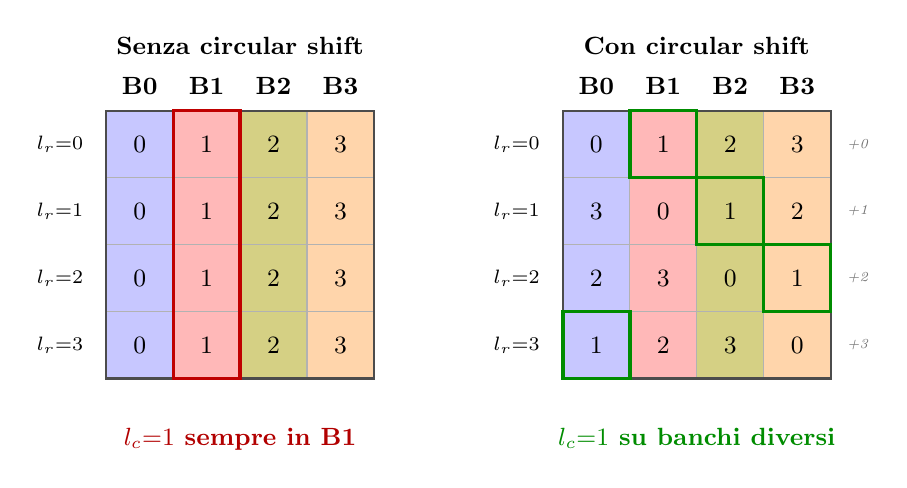
\begin{tikzpicture}[x=0.85cm, y=0.85cm]

%% === PANNELLO SINISTRO: senza circular shift ===
\fill[blue!22]   (0, 0) rectangle (1,-4);
\fill[red!28]    (1, 0) rectangle (2,-4);
\fill[olive!38]  (2, 0) rectangle (3,-4);
\fill[orange!33] (3, 0) rectangle (4,-4);

%% Contenuto cella = indice di colonna virtuale (= fisico, senza shift)
\foreach \r in {0,...,3} {
    \foreach \c in {0,...,3} {
        \node[font=\small] at (\c+0.5,-\r-0.5) {\c};
    }
}

\foreach \c in {0,...,4} \draw[gray!60, thin] (\c,0)--(\c,-4);
\foreach \r in {0,...,4} \draw[gray!60, thin] (0,-\r)--(4,-\r);
\draw[black!70, thick] (0,0) rectangle (4,-4);

%% Colonna virtuale l_c=1: striscia verticale in B1
\draw[red!75!black, very thick] (1,0) rectangle (2,-4);

\foreach \b/\c in {0/0,1/1,2/2,3/3}
    \node[above, font=\small\bfseries] at (\c+0.5, 0.1) {B\b};

\foreach \r in {0,...,3}
    \node[left, font=\scriptsize] at (-0.2,-\r-0.5) {$l_r{=}\r$};

\node[above, font=\small\bfseries] at (2, 0.7) {Senza circular shift};
\node[below, font=\small\bfseries, red!70!black, align=center] at (2,-4.6)
    {$l_c{=}1$ sempre in B1};

%% === PANNELLO DESTRO: con circular shift ===
\begin{scope}[xshift=5.8cm]

\fill[blue!22]   (0, 0) rectangle (1,-4);
\fill[red!28]    (1, 0) rectangle (2,-4);
\fill[olive!38]  (2, 0) rectangle (3,-4);
\fill[orange!33] (3, 0) rectangle (4,-4);

%% Contenuto cella = colonna virtuale al variare del shift
%% virtuale(li_r, phys_col) = (phys_col - li_r + 4) % 4
%% Riga 0 (shift=0): 0 1 2 3
\node[font=\small] at (0.5,-0.5) {0}; \node[font=\small] at (1.5,-0.5) {1};
\node[font=\small] at (2.5,-0.5) {2}; \node[font=\small] at (3.5,-0.5) {3};
%% Riga 1 (shift=1): 3 0 1 2
\node[font=\small] at (0.5,-1.5) {3}; \node[font=\small] at (1.5,-1.5) {0};
\node[font=\small] at (2.5,-1.5) {1}; \node[font=\small] at (3.5,-1.5) {2};
%% Riga 2 (shift=2): 2 3 0 1
\node[font=\small] at (0.5,-2.5) {2}; \node[font=\small] at (1.5,-2.5) {3};
\node[font=\small] at (2.5,-2.5) {0}; \node[font=\small] at (3.5,-2.5) {1};
%% Riga 3 (shift=3): 1 2 3 0
\node[font=\small] at (0.5,-3.5) {1}; \node[font=\small] at (1.5,-3.5) {2};
\node[font=\small] at (2.5,-3.5) {3}; \node[font=\small] at (3.5,-3.5) {0};

\foreach \c in {0,...,4} \draw[gray!60, thin] (\c,0)--(\c,-4);
\foreach \r in {0,...,4} \draw[gray!60, thin] (0,-\r)--(4,-\r);
\draw[black!70, thick] (0,0) rectangle (4,-4);

%% Colonna virtuale l_c=1: pattern diagonale
\draw[green!55!black, very thick] (1, 0) rectangle (2,-1);   % riga0, B1
\draw[green!55!black, very thick] (2,-1) rectangle (3,-2);   % riga1, B2
\draw[green!55!black, very thick] (3,-2) rectangle (4,-3);   % riga2, B3
\draw[green!55!black, very thick] (0,-3) rectangle (1,-4);   % riga3, B0

\foreach \b/\c in {0/0,1/1,2/2,3/3}
    \node[above, font=\small\bfseries] at (\c+0.5, 0.1) {B\b};

\foreach \r in {0,...,3}
    \node[left, font=\scriptsize] at (-0.2,-\r-0.5) {$l_r{=}\r$};

\foreach \r in {0,...,3}
    \node[right, font=\tiny, black!55] at (4.1,-\r-0.5) {\textit{+\r}};

\node[above, font=\small\bfseries] at (2, 0.7) {Con circular shift};
\node[below, font=\small\bfseries, green!55!black, align=center] at (2,-4.6)
    {$l_c{=}1$ su banchi diversi};

\end{scope}

\end{tikzpicture}
}
\caption{Layout fisico del tile $4\times4$ in fase~1. Ogni cella mostra l'indice di colonna virtuale ($l_c$) memorizzato in quella posizione fisica. I bordi evidenziati tracciano gli elementi con $l_c{=}1$, che vengono letti tutti simultaneamente in fase~2 con $l_r{=}1$ fisso. Senza circular shift cadono nella stessa colonna (B1); con circular shift ogni riga applica uno shift crescente (annotazioni \textit{+r} a destra), distribuendo $l_c{=}1$ su quattro banchi distinti.}
\label{fig:circular_layout}
\end{figure}

A differenza del padding, l'indirizzamento circolare non richiede alcuna memoria aggiuntiva e lascia inalterata l'occupancy. Il calcolo di \texttt{circular\_index} introduce una sola addizione e un confronto per work-item, un costo trascurabile rispetto ai guadagni. Le prestazioni risultanti sono molto vicine a quelle del kernel \texttt{init}.